\section{考察}
結果として以下のような形でPCからは映像の出力が得られるようになった.操縦者はPC上に描画される映像を元に操縦することで機体の操縦に集中しながら注意すべき対象が前方にある場合には強調して表示されるシステムが完成した.
\begin{figure}[htbp]
  \begin{center}
    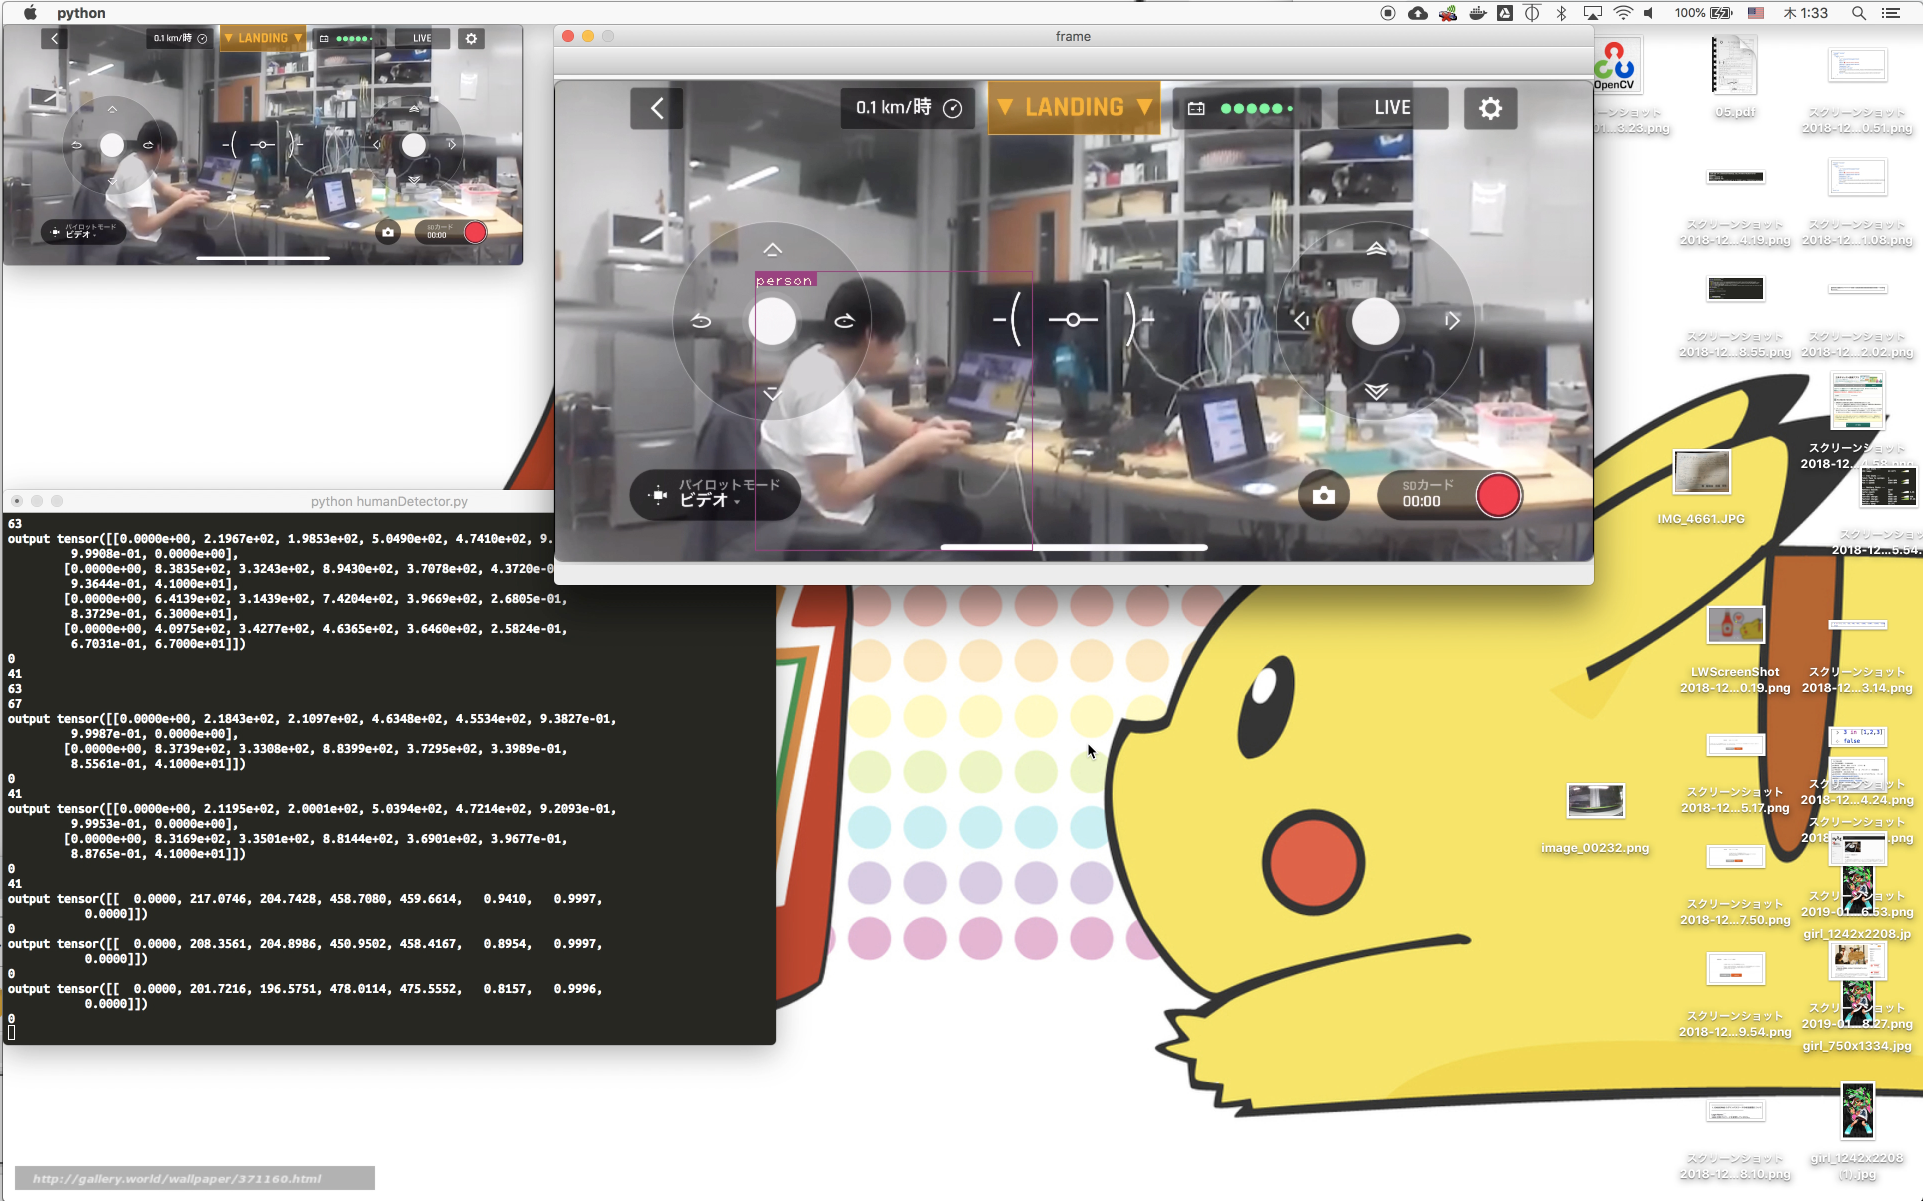
\includegraphics[clip,width=7.0cm]{img/sys-image.png}
    \caption{PC上の表示}
    \label{fig:sys}
  \end{center}
\end{figure}


しかし,現在の状態ではCPUの演算能力でのみ物体検知を行っており,2~3FPSしか計算ができていない.
この数値では実際に違和感なく操縦をするには物足りない結果である.
実験としては良いものの,実用にはまだまだ耐えられないものという結果になった.

この原因として考えられるのが現在物体検知モデルを動作させている環境でうまくGPUを利用することができておらず,これが一番の原因であると考えられる.
今後別環境での同システムの構築,検証が求められる.


また,このシステムを用いての定量的な評価も取れていない為,今後定量評価の為の環境も構築する必要がある.
